\documentclass[sigconf,anonymous]{acmart}
\settopmatter{printacmref=false}
\setcopyright{none}
\renewcommand\footnotetextcopyrightpermission[1]{}
\pagestyle{plain}

\usepackage{booktabs}

\newcommand{\Rl}{R(\ell)}
\newcommand{\Gl}{G(\ell)}

\acmConference[ICAIF '26]{7th ACM International Conference on AI in Finance}{November 2026}{}
\acmYear{2026}

\begin{document}

\title{Does a Learned Market Simulator React? Causal Injection Tests Against the Impact Kernel}

\author{Anonymous Author(s)}
\affiliation{\institution{Anonymous Institution}\city{}\country{}}

\begin{abstract}
Backtests that replay recorded market data cannot account for market impact, because the recording never reacts to the strategy under test. Generative models of order flow promise to close this gap, but published evaluations of their reactivity are distributional or coarse; to our knowledge, none isolates the causal effect of a single exogenous order against a quantitative magnitude reference. We propose a causal evaluation protocol. A single trade the model never generated is injected into real context, buy and sell arms are rolled out under positional common random numbers that share sampling noise across arms at every output position, and the paired response is graded against the impact kernel deconvolved from the order-sign autocorrelation under the propagator model. The benchmark is essential; on our data the single-trade kernel is roughly an order of magnitude smaller than the raw response, so an evaluation against the wrong reference would misjudge a correct simulator severalfold. We apply the protocol to an 87M-parameter autoregressive transformer trained on Binance perpetual-futures order flow, with results from a test split used for neither training nor checkpoint selection. Across 2{,}048 paired injections per symbol, the buy--sell contrast is positive through at least lag 75 on every symbol at both injected order sizes, while the plateau comparison against each symbol's kernel discriminates sharply. SOL passes the pre-declared factor-two equivalence test at both order sizes with kernel uncertainty propagated (ratio intervals $[0.68, 1.42]$ and $[0.94, 1.71]$), ETH's median-size response is positive but attenuated and its large-order response inverts sign, and BTC, a negative control, responds wrong-signed at both order sizes. A TWAP execution study quantifies the practical consequence. The reactive simulator charges 0.33--0.72 ticks per unit of quote-response cost that replay scores as zero. We argue that injection tests against the impact kernel should become a standard evaluation for learned market simulators.
\end{abstract}

\begin{CCSXML}
<ccs2012>
<concept>
<concept_id>10010405.10010481.10010485</concept_id>
<concept_desc>Applied computing~Economics</concept_desc>
<concept_significance>500</concept_significance>
</concept>
<concept>
<concept_id>10010147.10010257</concept_id>
<concept_desc>Computing methodologies~Machine learning</concept_desc>
<concept_significance>500</concept_significance>
</concept>
</ccs2012>
\end{CCSXML}
\ccsdesc[500]{Applied computing~Economics}
\ccsdesc[500]{Computing methodologies~Machine learning}

\keywords{market simulation, limit order books, generative models, market impact, causal evaluation, backtesting}

\maketitle

\section{Introduction}

A typical backtest evaluates a candidate strategy by replaying recorded market data against it. The recording, however, never reacts. The strategy's fills are free, and the recorded price path is unaffected by any order the strategy submits. For strategies that trade meaningful size this is a severe deficiency, because the quantity a backtest most needs to estimate, the effect of the strategy's own trading on the price, is zero by construction.

Generative models of order flow offer a solution. A model trained to predict the next market event given history yields rollouts that constitute a synthetic market capable, in principle, of reacting. Once an injected order enters the model's context, everything generated afterwards is conditioned on it. A rapidly growing literature builds such simulators from GANs \citep{coletta2021,coletta2022}, autoregressive token models \citep{nagy2023}, masked-language-model encoders \citep{lobert2025}, diffusion models \citep{trades2025,difflob2026}, and order-level foundation models \citep{mars2025}.

Evaluation has not kept pace. The standard tests are distributional, comparing spreads, volumes, inter-arrival times, and return moments between generated and real data \citep{cont2001,lobbench2025}. These are necessary conditions, but they cannot certify reactivity. A simulator can match every marginal and still respond incorrectly to an exogenous order, because distributional statistics are computed on rollouts in which the model only ever responds to its own flow. Where responsiveness is tested at all, the tests are coarse. A percentage-of-volume agent is activated and the resulting mid-price difference plotted \citep{coletta2022,trades2025}, or synthetic impact is calibrated to aggregate impact laws \citep{mars2025,noble2026}. None of these designs isolate the causal effect of a single exogenous order, and none compare the measured response to the quantity that microstructure theory predicts for one.

That quantity exists. Because order signs have long memory \citep{lillofarmer2004}, the average price move following a buy is the combined impact of the buy and the correlated buys that typically accompany it. The propagator model \citep{bouchaud2004,taranto2016} separates the two. The observed (dressed) response $\Rl$ is the single-trade impact kernel $\Gl$ convolved with the sign autocorrelation, so measurements of $\Rl$ and the sign autocorrelation identify $\Gl$ by deconvolution. An injected trade in a simulator is precisely an exogenous, uncorrelated trade, and its response should therefore be compared to the impact kernel rather than the dressed response. On our data the two differ by more than an order of magnitude.

\paragraph{Contributions.} We propose and demonstrate a causal evaluation protocol for learned market simulators:
\begin{enumerate}
\item \textbf{Paired injection tests under positional common random numbers.} A single marketable order the model never generated is spliced into real context, and buy and sell arms are rolled out sharing their sampling noise at every position via Gumbel-argmax sampling, so that the paired difference $(R_{\mathrm{buy}}-R_{\mathrm{sell}})/2$ is a causal contrast between the two intervention signs and the pairing survives arbitrary divergence of the token histories, at an unchanged marginal sampling law.
\item \textbf{The impact kernel as a direct-effect reference.} We deconvolve the impact kernel from real trades under the propagator model. Because an exogenous trade may legitimately induce reaction, the primary structural prediction, derived from the propagator assumptions rather than guaranteed by them, is a bracketing, $G \le \hat{R}_{\mathrm{inj}} < R$. Closeness to $G$ is a secondary direct-effect calibration with pre-declared equivalence margins.
\item \textbf{A negative control by construction.} We run the identical protocol on a symbol selected as a negative control because independent distributional diagnostics indicate excess trend persistence. Its failure demonstrates that the protocol discriminates rather than mechanically producing favorable outcomes.
\item \textbf{The replay gap.} A TWAP execution strategy evaluated in replay, in the reactive simulator, and against a no-trade control identifies a quote-response cost of 0.33--0.72 ticks per unit that replay scores as zero.
\end{enumerate}

The demonstration vehicle is an 87M-parameter decoder-only transformer trained on raw Binance perpetual-futures order flow (Section~\ref{sec:model}). To our knowledge this is the first learned LOB simulator built and evaluated on cryptocurrency perpetual L2 data. The methodology itself is model-agnostic. Any generative order-flow model that can accept an injected event can be evaluated in the same way.

\section{Related work}
\label{sec:related}

\paragraph{Learned LOB simulators.} \citet{jain2024} survey the field, which spans hand-calibrated agent-based simulation \citep{abides2019}, hybrid neural agents \citep{shi2023}, whose evaluation includes percentage-of-volume (POV) agent experiments contrasting responsive and non-responsive background flow, and fully learned generators. \citet{coletta2021,coletta2022} train a conditional-GAN ``world agent'' on historical flow, evaluated with a stylized-fact battery and a POV-agent injection measured as the average mid-price difference with and without the agent. \citet{nagy2023} introduce the first end-to-end autoregressive token-level generative model of LOB messages and name realistic market impact as an open problem. LOBERT \citep{lobert2025} adapts a BERT-style foundation model to LOB messages, evaluated on prediction accuracy and marginal fidelity. TRADES \citep{trades2025}, a diffusion generator, demonstrates responsiveness qualitatively through a single POV-agent experiment. DiffLOB \citep{difflob2026} diagnoses the same passivity problem we target, observing that prior generative LOB models ``remain fundamentally passive'', but intervenes at the level of market regimes rather than individual orders. MarS \citep{mars2025} is the closest system-level work, an order-level autoregressive foundation model demonstrated as an interactive simulator with a TWAP-agent experiment and a square-root-law check. \citet{noble2026} build an interactive simulator with an explicit, calibrated impact-feedback term validated against impact laws rather than by intervention on a learned generator.

\begin{table}[t]
\centering
\small
\begin{tabular}{p{2.45cm}p{4.9cm}}
\toprule
Work & Responsiveness evaluation \\
\midrule
\citet{coletta2021,coletta2022} & POV agent; mean mid-price difference \\
\citet{nagy2023} & none (impact named as open problem) \\
\citet{trades2025} & POV agent; qualitative \\
\citet{mars2025} & TWAP demo; square-root-law check \\
\citet{difflob2026} & regime-level counterfactuals \\
\citet{lobbench2025} & $\Rl$ on free rollouts; no injection \\
\citet{noble2026} & calibration to impact laws \\
\midrule
This work & paired single-trade injection, positional CRN, dose scaling, kernel match, falsification \\
\bottomrule
\end{tabular}
\caption{How reactivity is evaluated across LOB simulators. To our knowledge, no prior work injects a single exogenous trade under paired common-random-number arms or compares the response to the deconvolved impact kernel.}
\label{tab:related}
\end{table}

\paragraph{Evaluation methodology.} LOB-Bench \citep{lobbench2025} is the emerging standard benchmark. It is explicitly distributional, measuring L1 and Wasserstein-1 divergences plus discriminator scores on US-equity LOBSTER data. Its impact metrics, including $\Rl$, are computed on freely generated sequences, not under intervention, and its authors flag testing generated impact against impact laws as future work. Our protocol is complementary. Distributional batteries assess unconditional behavior; injection tests assess the causal response to exogenous orders.

\paragraph{Impact theory.} The propagator model \citep{bouchaud2004}, the long memory of order signs \citep{lillofarmer2004,lmf2005}, and their joint implications for response functions \citep{bouchaud2009,taranto2016,gatheral2010} provide the theory behind our metrics. The square-root law \citep{toth2011} concerns metaorders executed against daily volume; Section~\ref{sec:replaygap} shows why it is the wrong benchmark for second-scale single-trade experiments. \citet{naviglio2025} show that price models calibrated on public data typically get metaorder impact qualitatively wrong, motivating evaluation on exactly this axis.

\section{Data, representation, and model}
\label{sec:model}

\paragraph{Corpus.} We use Binance USD-margined perpetual-futures incremental L2 depth and trade feeds from Tardis.dev. The corpus comprises 198 training symbol-days of BTCUSDT, ETHUSDT, and SOLUSDT spanning 2021 through mid-2026, plus one held-out day per symbol. Binance publishes depth diffs on a fixed $\sim$26\,ms timer, so book updates carry no event-time process of their own; event-time structure resides in the trades. A median frame carries 25 level changes, the book is consistent only at frame boundaries, and a single day of BTC perpetual L2 alone contains 161M book events.

\paragraph{Tokenization.} The representation is a single chronological stream. Every event opens with a log-bucketed $\Delta t$ token, followed by either a trade (side, price offset, size) or a frame (a list of near-touch level changes). Price offsets are expressed in ticks from the pre-event same-side best, so generated events can be applied forward without self-reference; in-band offsets cover $-16$ to $+63$, and a two-digit base-32 jump escape encodes larger price improvements exactly up to 1,040 ticks. The escape matters for backtesting realism; improvements beyond the in-band range occur on 0.8\% of frames on a calm day and 3.2\% on a violent one, and the largest observed frame moved 34,545 ticks, so representation failures concentrate exactly where a backtesting simulator matters most, in the tails. Sizes use 32 log$_2$ buckets. All buckets are fixed a priori, so the tokenizer involves no fitting to data. The vocabulary is 384 tokens, an event averages $\sim$2.6 tokens, and the corpus contains 11.75B tokens.

\paragraph{Model.} The model is a decoder-only transformer with 87M parameters, width 768, 12 layers, 12 heads, and a context of 2,048 tokens ($\sim$10--13\,s of market), trained with Muon (learning rate $2\times10^{-2}$). Validation loss selects the checkpoint at step 22{,}000 ($\sim$1.44B token presentations), which reaches 1.375 nats/token on a strictly walk-forward validation set; the uniform baseline is $\ln 384 = 5.95$. Decoding is grammar-constrained, masking any token that would be syntactically illegal at the current position; the raw probability mass on illegal tokens is only 0.05--0.07\% per step.

\section{Distributional evaluation}
\label{sec:distributional}

Before asking whether the simulator reacts, we ask whether its free-running output is statistically realistic. Here and throughout, the evaluation discipline is the same. The holdout day is split in half; the first (validation) half was used for checkpoint selection and protocol development, and the second (test) half supplies every statistic reported in this paper. We seed the model with 2,048 tokens of real test-split context, roll out, and compare rollouts to test-split real data on spread and depth distributions (by Kolmogorov--Smirnov distance), event rates, crossed books, kurtosis decay, volatility clustering, and the variance signature plot.

\paragraph{A real-vs-real noise floor.} A KS distance of 0.1 is not interpretable in isolation, since even two disjoint windows of \emph{real} market data do not have identical distributions. We therefore compute each metric between two disjoint real windows and use this real-vs-real value as a noise floor. Pooled across symbols, the spread KS passes below the noise floor, but the pass is an artifact of cross-symbol composition; stratified by symbol, spread realism is mixed (Table~\ref{tab:scorecard}). Distributional evaluations of multi-asset generative models should always be stratified.

\begin{table}[t]
\centering
\small
\begin{tabular}{lccc}
\toprule
generated (real) & BTC & ETH & SOL \\
\midrule
frames/s & 33.0 (35.9) & 38.7 (39.6) & 34.5 (32.9) \\
trades/s & 39.2 (60.7) & 154.4 (70.3) & 57.1 (31.2) \\
spread KS (floor) & 0.18 (0.10) & 0.015 (0.000) & 0.13 (0.29) \\
crossed per 1k (base) & 12.9 (10.7) & 13.9 (0.0) & 1.0 (0.0) \\
illegal mass per step & 0.05\% & 0.05\% & 0.06\% \\
\bottomrule
\end{tabular}
\caption{Stratified scorecard on the held-out test split (four 12k-token rollouts per symbol). Frame timing is close on all symbols, but generated trade rates run high on ETH and SOL, and ETH's spread tail occasionally blows out. Free-running realism on the test half is imperfect, which sharpens the question of whether causal responses survive.}
\label{tab:scorecard}
\end{table}

\begin{figure*}[t]
\centering
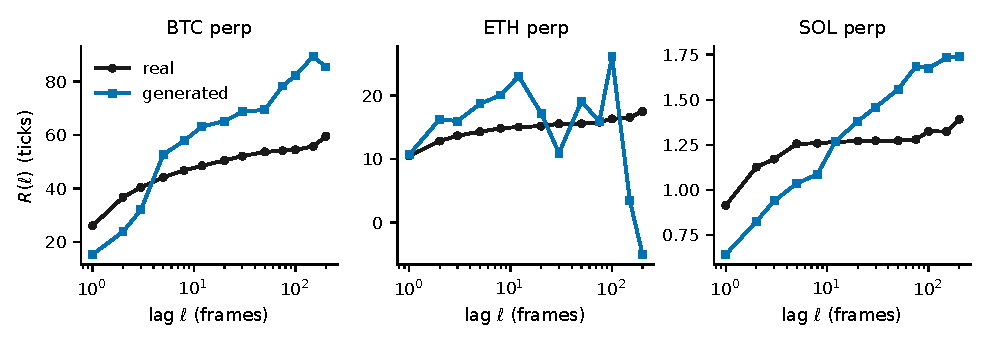
\includegraphics[width=\textwidth]{figures/impact.pdf}
\caption{Impact response function $\Rl$, real vs.\ generated, per symbol (lags in $\sim$26\,ms frames). Impact is emergent; nothing in training targets it. Short-lag magnitude and shape are close on all symbols; generated impact fails to plateau, most severely on BTC.}
\label{fig:impact}
\end{figure*}

\begin{figure*}[t]
\centering
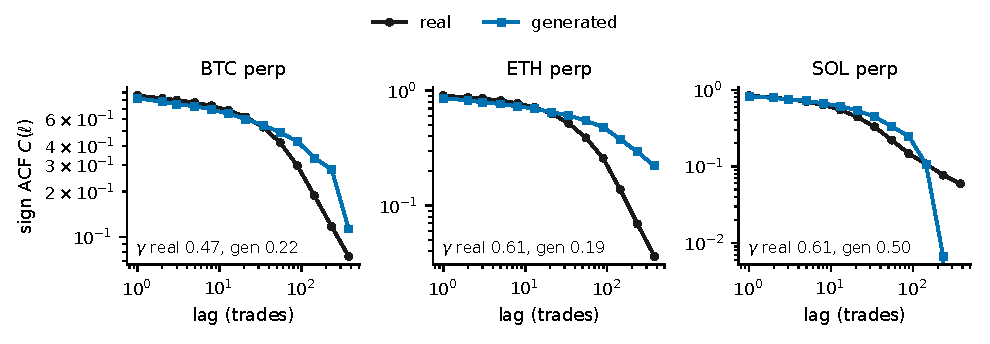
\includegraphics[width=\textwidth]{figures/signacf.pdf}
\caption{Order-sign autocorrelation, log--log. Generated flow (blue) is more persistent than real (black) on every symbol; the $\gamma$ gap is largest on ETH (0.42) and smallest on SOL (0.10).}
\label{fig:signacf}
\end{figure*}

\paragraph{Emergent impact, over-persistent flow.} The first economic metric is the response function $\Rl = \mathbb{E}[\epsilon \cdot (m_{t+\ell}-m_t)]$, the average signed mid-price move following a trade. Although nothing in next-token training targets impact, the generated market reproduces the shape and short-lag magnitude of the real response on all three symbols (Figure~\ref{fig:impact}). The systematic failure appears at long lags. Real impact plateaus, whereas generated impact continues to climb, exceeding the real value by roughly 50\% at lag 100 on BTC and ETH. The mechanism is over-persistent order flow. Real order signs decay as $C(\ell)\sim\ell^{-\gamma}$ \citep{lillofarmer2004} with $\gamma = 0.47/0.61/0.61$ on BTC/ETH/SOL, against generated $0.22/0.19/0.50$ (Figure~\ref{fig:signacf}). Generated flow is too persistent on every symbol, with the memory gap smallest on SOL (0.10) and largest on ETH (0.42); in a market with transient impact, over-persistent flow prevents the response from plateauing. These results set the stage. Free-running realism on the test split is imperfect and strongly symbol-dependent, with ETH degrading the most, and, as Section~\ref{sec:results} shows, the causal picture is not what the distributional picture suggests.

\section{Injection methodology}
\label{sec:method}

The distributional battery leaves one question unanswered. Does the model treat an exogenously submitted order as information? Nothing in next-token training guarantees that it treats an exogenous trade as anything but noise.

\paragraph{Design.} We take 2{,}048 windows of real test-split context per symbol (1,532 tokens each, cut at event boundaries, spanning each symbol's test region). For each window we run five arms sharing the identical context, a marketable buy at the touch and a marketable sell at the touch, each at two doses, the median trade size ($1\times$) and three size buckets larger ($\approx 8\times$), plus a no-injection control. The injected trade is spliced in as four tokens ($\Delta t$, side, offset~0, size). Each arm then generates 2,500 new tokens, so the buy and sell rollouts differ by exactly one token of input, and the paired statistic $\hat{R}_{\mathrm{inj}}(\ell) = \tfrac{1}{2}(R_{\mathrm{buy}}(\ell) - R_{\mathrm{sell}}(\ell))$ is a causal contrast between the two intervention signs; it equals the effect of a buy relative to no order only under buy/sell antisymmetry, which we test rather than assume. The control arm measures residual drift. A bookkeeping check verifies that each spliced trade is parsed as intended and that the rollout reaches the plateau window; valid pairs number 1{,}991 and 1{,}997 of 2{,}048 at the two doses on SOL, 1{,}998 and 1{,}997 on ETH, and 2{,}021 and 2{,}017 on BTC. Confidence intervals are 95\% percentile bootstraps over seeds (2{,}000 resamples) unless noted; equivalence tests use 90\% intervals as the two-one-sided-test construction requires.

\paragraph{Positional common random numbers.} Pairing gives the contrast its power, and ordinary common random numbers pair imperfectly. With a shared-seed sampler, the coupling between the arms' emitted tokens weakens once their histories diverge. We instead sample each token by Gumbel-argmax. For window $w$, a per-window noise stream advanced once per output position yields a vocabulary-sized Gumbel vector $g_{w,t}$ that is a deterministic function of $(w,t)$ alone, and the emitted token is $\arg\max_v (z_v/T + g_{w,t,v})$ over the grammar-legal logits $z$. Per position this reproduces exactly the masked softmax sampling law, so each rollout's marginal distribution is unchanged, but because the noise is indexed by position rather than by sampling history, all five arms share their entire noise realization no matter how far their token streams diverge. On our data this cuts the variance of the paired plateau statistic roughly in half relative to shared-seed sampling, at no cost in generation.

\paragraph{Criteria fixed in advance.} \emph{Sign}: the paired response must be positive with confidence intervals clear of zero. \emph{Dose}: the $8\times$ injection must produce a larger response than $1\times$. \emph{Magnitude}: the response must be quantitatively right. The magnitude test is scored in the kernel's plateau window (trade lags 16--24, where the real $G$ has flattened) as the per-seed mean over those lags, bootstrapped across seeds, and formalized as a two-one-sided equivalence test with margins declared before any test-split data was analyzed, a primary margin of a factor of two around the kernel and a secondary margin of 1.5.

\paragraph{The magnitude yardstick.} The natural candidate is the measured response to real trades, $R(\ell)$, but it is the wrong target. Real order flow is autocorrelated ($C(1)=0.840$ on SOL), so $R(\ell)$ prices the correlated flow that accompanies a real trade, while an injected trade carries no such flow. Under the propagator model \citep{bouchaud2004,taranto2016}, $m_i = \sum_{j<i} G(i-j)\,\epsilon_j + \eta_i$, which implies the linear system
\[
R(\ell) = \sum_{m\ge 1}\big[C(|m-\ell|)-C(m)\big]\,G(m),
\]
truncated at $m \le L$ and solved by least squares for $G$. We do this per symbol on 336k--504k real test-split trades, on the trade clock, with $L=64$; uncertainty comes from a segment bootstrap (twelve $10^6$-token segments, re-pooling $\hat R$ and $\hat C$ jointly before deconvolving), since the square system's residual is numerical rather than statistical. The deconvolved kernels plateau at $+0.032$ ticks on SOL, $+0.175$ on ETH, and $+0.423$ on BTC, in each case more than an order of magnitude below the dressed response at the same lags. Identification quality differs sharply. A truncation sweep over $L \in \{32,\dots,64\}$ and a ridge sweep move the SOL kernel by under 20\% (segment bootstrap $[0.027, 0.036]$), the ETH kernel by 60\% at the shortest horizon, and the BTC kernel by a factor of $2.2$, so the BTC kernel is at best loosely identified. One caution governs interpretation. Deconvolution removes correlated future flow whether that flow is confounding or a genuine reaction the trade causes, so $G$ is a \emph{direct-effect} reference rather than the unique causal truth. The total response to an exogenous trade may legitimately exceed $G$ through induced reaction, while the fully dressed $R$ prices the entire historical correlated crowd. Under the propagator assumptions, with a nonnegative kernel and induced flow no stronger than the historical correlated flow, the response is predicted to fall between the two,
\[
G_{\mathrm{real}} \;\le\; \hat{R}_{\mathrm{inj}} \;<\; R_{\mathrm{real}},
\]
a structural diagnostic under those stated assumptions rather than a bound that cannot be violated, with closeness to $G$ as a secondary calibration.

\begin{figure*}[t]
\centering
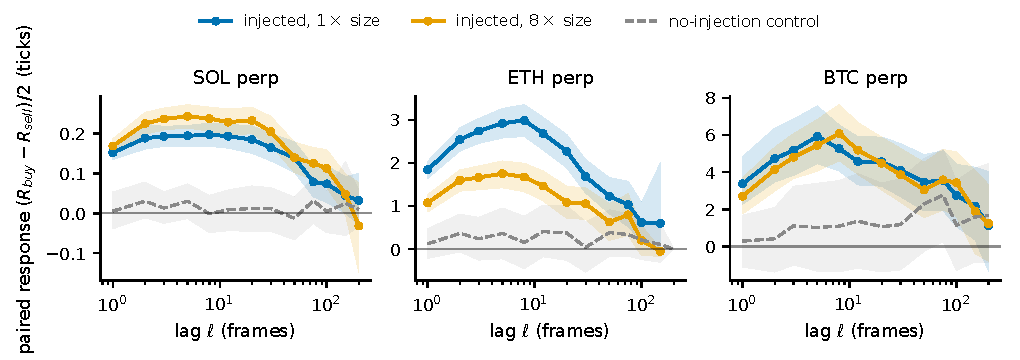
\includegraphics[width=\textwidth]{figures/injection.pdf}
\caption{Paired injection response on the held-out test split, with bootstrap 95\% bands, 2{,}048 seeds per symbol; note the differing y-scales. The frame-clock response is positive with intervals clear of zero through at least lag 75 on every symbol at both doses, so at these lags the sign criterion does not discriminate; the trade-clock plateau comparison of Figure~\ref{fig:plateau} does. The no-injection controls are consistent with zero at every lag on SOL and ETH; BTC's control drifts positive at lag 75 (pointwise).}
\label{fig:injection}
\end{figure*}

\section{Injection results}
\label{sec:results}

\paragraph{Sign.} On the frame clock the paired buy-minus-sell response is positive with bootstrap intervals clear of zero through lag 100 on SOL at both doses, through lag 100 at $1\times$ and lag 75 at $8\times$ on ETH, and through lag 150 at $1\times$ and lag 100 at $8\times$ on BTC (Figure~\ref{fig:injection}); at short and intermediate lags the sign criterion does not discriminate among the symbols. The control arms are consistent with zero at every measured lag on SOL and ETH; BTC's control is positive at lag 75 ($2.8$ $[0.3, 5.3]$, pointwise), a further sign of its instability. Injection leaves the model's syntax undisturbed, and the spread and crossed-frame marginals of injected rollouts remain of the same order as the control arm's, although BTC deteriorates in the upper tail (90th-percentile spread 2.6 ticks in control against 2.8--3.2 injected). The discrimination appears at the trade-clock plateau.

\paragraph{Dose.} An $8\times$ order should not be expected to produce an $8\times$ response. The size-conditioned response of real trades is nearly flat (Section~\ref{sec:replaygap}), so the causal response should grow far more slowly than proportionally. On SOL the paired dose difference is $+0.008$ $[-0.005, +0.019]$, consistent with both zero and a shallow dependence; the pre-declared dose criterion, a strictly larger response at $8\times$, is therefore not established even where everything else passes. On ETH the large dose \emph{fails}. The paired dose difference is $-0.173$ $[-0.254, -0.092]$, significantly negative, and the $8\times$ response itself is wrong-signed ($-0.059$, with a 95\% interval $[-0.120, -0.0003]$ that only marginally excludes zero, but a temporal-block interval $[-0.108, -0.016]$ that excludes it clearly). A plausible mechanism is that the injected size bucket is rare in ETH's flow, leaving the large injection partially out of distribution. This failure is invisible to distributional evaluation and is precisely the kind of defect the protocol exists to catch.

\begin{figure*}[t]
\centering
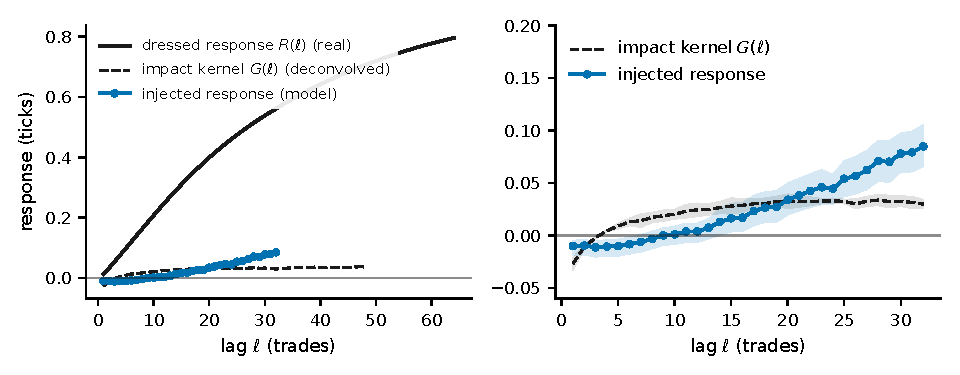
\includegraphics[width=\textwidth]{figures/kernel.pdf}
\caption{Dressed response, impact kernel, and injected response (SOL, trade-clock lags, test split). Left: the dressed response $R(\ell)$ to real trades dwarfs both the deconvolved impact kernel $G(\ell)$ and the model's injected response; comparing injections to $R$ would misjudge the simulator by an order of magnitude. Right: zoomed. The injected response (blue, 95\% bootstrap band) runs at the kernel's scale.}
\label{fig:kernel}
\end{figure*}

\begin{figure}[t]
\centering
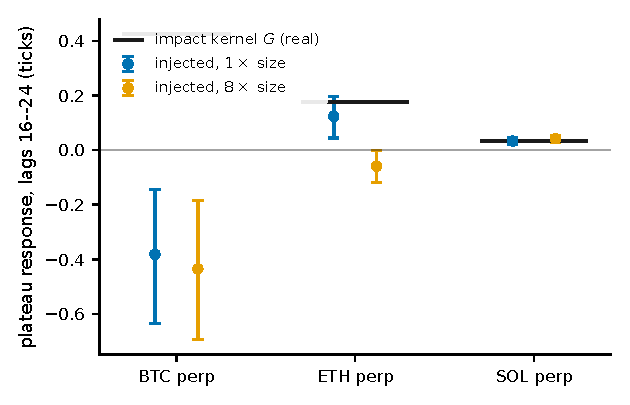
\includegraphics[width=\columnwidth]{figures/plateau.pdf}
\caption{The magnitude test (2{,}048 seeds). Per-seed plateau-window (trade lags 16--24) injected response with 95\% bootstrap intervals, against the impact kernel deconvolved from each symbol's real trades (black bars). SOL passes factor-two equivalence at both doses; ETH's median-size response falls below its kernel at the point estimate and its large-dose response inverts sign; BTC is significantly wrong-signed at both doses. BTC's kernel itself is only loosely identified.}
\label{fig:plateau}
\end{figure}

\paragraph{Magnitude.} Figures~\ref{fig:kernel} and~\ref{fig:plateau} present the central result. On SOL the plateau response is $+0.033$ $[+0.019, +0.046]$ at $1\times$ and $+0.042$ $[+0.029, +0.054]$ at $8\times$ against a kernel of $+0.032$, point estimates at $1.0$ and $1.3\times$ the kernel, inside the predicted bracket $[G, R)$, and stable under temporal-block resampling. Formal equivalence at the pre-declared factor-two margin is established at both doses. With kernel uncertainty propagated by a ratio bootstrap (response draws over kernel draws, kernel draws recentred on the propagator-plateau kernel so that numerator and denominator agree in expectation), the SOL ratio intervals are $[0.68, 1.42]$ at $1\times$ and $[0.94, 1.71]$ at $8\times$, both inside $[1/2, 2]$, and the $1\times$ interval also passes the stricter secondary margin of 1.5. On ETH the median-size plateau response is positive ($+0.123$ $[+0.044, +0.196]$) but attenuated. The point estimate is $0.71\times$ its kernel of $+0.175$, and the 90\% ratio interval $[0.33, 1.06]$ establishes neither equivalence at either margin nor a resolved deficit, so the bracketing fails from below at the point-estimate level while the sample leaves the under-reaction short of significance. Nothing in training targets these quantities; they emerge from next-token prediction on raw flow. Under the three pre-specified criteria, SOL passes sign and magnitude while its dose criterion remains unestablished; ETH and BTC fail. The supported claim is formal factor-two equivalence on SOL and point-estimate attenuation, without a statistically resolved deficit, on ETH.

\paragraph{Induced flow, and what the estimand is.} The model interprets a single exogenous trade as part of a metaorder. The paired buy--sell contrast in the sign of the next generated trade is $+0.43$ on SOL, $+0.57$ on ETH, and $+0.42$ on BTC, decaying over tens of trades. This induced herding is why the SOL response sits at or above the impact kernel within the bracket. Two caveats delimit the estimand. First, the paired statistic is a causal contrast between buy and sell interventions rather than a buy-versus-no-order effect; decomposed against the control arm, all four SOL single-arm effects are individually significant with the correct signs (at $1\times$, buy $+0.030$ $[+0.004, +0.054]$ and sell $-0.035$ $[-0.064, -0.009]$), whereas ETH's decomposition is asymmetric. At $1\times$ the sell arm carries the effect ($-0.177$ $[-0.307, -0.033]$) and at $8\times$ the buy arm is itself significantly wrong-signed ($-0.124$ $[-0.236, -0.018]$). Second, the buy/sell antisymmetry that would equate the contrast with twice the single-arm effect is consistent with zero in all six symbol-dose cells.

\paragraph{BTC as a negative control.} A passing result is informative only if the test is capable of failing, so we include BTC as a selected negative control. Its generated flow independently exhibits severe sign-memory excess and non-plateauing impact on the distributional battery (Section~\ref{sec:distributional}), so the distributional diagnostics predict failure before any injection is run. The test fails at both doses. The plateau response is significantly wrong-signed at $1\times$ ($-0.38$ $[-0.64, -0.15]$) and at $8\times$ ($-0.43$ $[-0.69, -0.18]$), both retained under temporal-block resampling; an injected buy \emph{lowers} the mid at plateau horizons while the frame-clock response reads positive, so the response is internally contradictory across clocks. The deterioration is driven by the buy arms (at $8\times$, buy-minus-control is $-0.94$ $[-1.84, -0.13]$). A simulator whose causal response is wrong-signed where it is measurable cannot support agent evaluation. The instrument discriminates; that is the purpose of the negative-control arm.

\paragraph{Distributional health does not determine causal quality.} A natural hypothesis is that the sign-memory gap orders injection outcomes. On this data the association is directionally present but coarse. SOL, with the smallest gap ($0.10$), is the only symbol whose response certifies equivalence to its kernel, while ETH ($0.42$) and BTC ($0.25$) both fail, but in qualitatively different ways the gap does not predict. ETH responds at $0.7\times$ its kernel at median size and inverts at large dose while keeping the correct frame-clock sign, whereas BTC's plateau is wrong-signed beneath a healthy-looking frame-clock response. Free-running diagnostics alone would reveal neither failure mode.

\section{Quantifying the replay gap}
\label{sec:replaygap}

\paragraph{Design.} The strategy is a TWAP taker that must buy a fixed quantity on SOL as $K=8$ marketable child orders at the touch, spaced 250 generated tokens apart. We evaluate it over 256 seeds in three ways: under \emph{naive replay}, where fills occur at recorded prices and the market cannot react; under the \emph{reactive} simulator, where each child order is injected and generation continues from it; and against a \emph{no-trade control} in the same generated market under common random numbers. Execution cost is implementation shortfall (mean child fill price minus arrival mid, ticks per unit), and self-caused impact is the reactive shortfall minus the control shortfall. Child size sweeps $\tfrac{1}{8}\times$ to $64\times$ the median trade size. One mechanical limitation defines what is measured. Injected child orders are filled at the prevailing best ask without consuming book depth, so the measured cost is the generated market's \emph{quote response}, a lower bound on total impact cost.

\begin{figure*}[t]
\centering
\begin{minipage}[t]{0.44\textwidth}
\centering
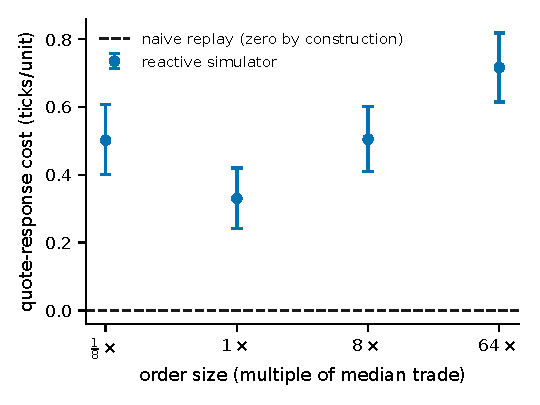
\includegraphics[width=0.82\textwidth]{figures/pnlgap.pdf}
\end{minipage}\hfill
\begin{minipage}[t]{0.44\textwidth}
\centering
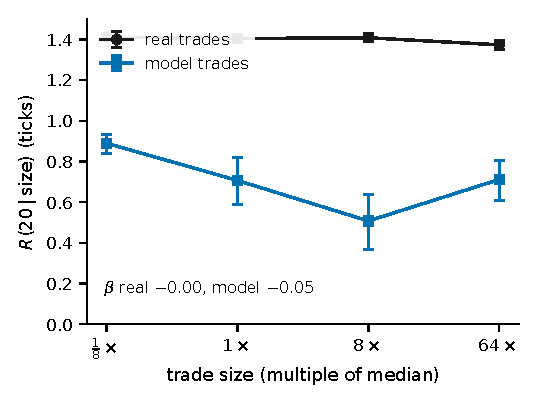
\includegraphics[width=0.82\textwidth]{figures/size.pdf}
\end{minipage}
\caption{Left: the replay gap on the test split. Naive replay charges zero impact by construction; the reactive simulator charges a quote-response cost of 0.33--0.72 ticks per unit (95\% CIs, 256 seeds), largest at the largest dose and non-monotone at small doses. Right: validating the flat size dependence against reality. The size-conditioned response to \emph{real} SOL trades is flat across a 512$\times$ size range (exponent $-0.004$); the model's own trades reproduce the flatness at a level roughly half the real one.}
\label{fig:pnl}
\end{figure*}

\paragraph{Replay understates a real cost.} Naive replay's impact is identically zero. The reactive simulator charges $+0.33$ to $+0.72$ ticks per unit across the dose range, every interval clear of zero (Figure~\ref{fig:pnl}). The cost is largest at the largest dose ($+0.72$ $[+0.62, +0.82]$ at $64\times$) but not monotone at small doses, so we do not fit a parametric size law. The robust statement is simpler. A replay backtest scores this entire cost, roughly half a tick per unit, as zero.

\paragraph{Flat size dependence reflects the data.} The square-root impact law \citep{toth2011} might suggest that nearly flat size dependence is a model failure. It is not. The law describes metaorders executed against daily volume, whereas this experiment probes single marketable orders over seconds \citep{bouchaud2009}. Measured identically on the real test split, the size-conditioned response is flat across a 512$\times$ size range (exponent $-0.004$); the model reproduces the flatness (exponent $-0.05$) at a level roughly half the real one, an error in the conservative direction. The conditional flatness partly reflects selection, since large real trades are placed when the book can absorb them.

\section{Limitations}
\label{sec:limits}

The scope is one venue, one asset class, and one calendar day, Binance perpetual futures across three symbols, with the test split being the second half of the day whose first half served for validation; cross-day and cross-venue generalization are untested. The 26\,ms frame cadence is the feed's ceiling and therefore the model's; only near-touch book state is modeled, sizes are log-bucketed, and trades see a book up to 26\,ms stale. The magnitude evidence certifies factor-two equivalence on SOL only, and the certification inherits every propagator-model assumption baked into the kernel. The reported intervals quantify within-run sampling uncertainty; variability across independent evaluation runs can exceed them. Injected orders enter as trade prints and do not consume book depth, so execution-cost figures are quote-response lower bounds; a matching engine with depth consumption is left to future work. The kernel is unstable at the first few lags (bid--ask bounce and near-collinearity with $C(1)$) and at the horizon edge, and response and kernel are estimated from the same trading day, with residual same-day dependence between them not modeled. Finally, validating the causal magnitude against real data is impossible in principle, because one cannot inject a trade into a recording. The deconvolved kernel is a model-based estimate of the causal quantity, not an experimental one. That impossibility is also the reason learned simulators are worth building, and it is precisely why their causal behavior must be tested rather than assumed.

\section{Conclusion}

A model trained only to predict the next token of order flow reacts causally to trades it never generated. On a held-out test split, the paired buy--sell contrast is positive for at least seventy-five frames on every symbol and dose, and on SOL the plateau response is formally equivalent to the impact kernel at the pre-declared factor-two margin at both doses, inside the predicted bracket between the kernel and the dressed response. The protocol's value is diagnostic as much as confirmatory. It exposes ETH's attenuated median-size response and large-dose sign inversion and the negative control's wrong-signed plateau, failures invisible to distributional evaluation. The practical consequence is measurable. Replay backtests omit a self-caused quote-response cost of 0.33--0.72 ticks per unit, itself a lower bound on full execution cost.

The broader argument is methodological. The field is converging on generative order-flow models as reactive backtesters but grades them almost entirely on distributional realism, which cannot certify the one property that reactive backtesting requires, a correct causal response to exogenous orders. Paired injection tests against the impact kernel are inexpensive, model-agnostic, and falsifiable, and we suggest that they join stylized facts and distributional benchmarks as standard evaluation for any simulator intended to support interactive strategy evaluation. Code and evaluation outputs will be released upon publication.

\bibliographystyle{ACM-Reference-Format}
\bibliography{refs}

\end{document}
